\section{Theoretical methods}
\label{sec:theory}

In this study, the vibrational and rotational spectroscopic investigations are
supported and complemented by quantum chemical calculations. Therefore, this
section briefly describes the quantum theory of molecular vibration and
rotation using a quantum mechanical approach.\\

In classical mechanics, the system's total energy, which includes kinetic ($T$)
and potential ($V$) energy, is known as the Hamiltonian ($H$), such that

\begin{equation}
    \label{eqn:classical:Hamiltonian}
    H = T + V
\end{equation}

Schr\"odinger postulated the form of Hamiltonian (operator) in quantum
mechanics, as given below

\begin{equation}
    \label{eqn:quantum:Hamiltonian}
    H = - \frac{\hbar^2}{2m} \nabla^2 + V(r)
\end{equation}

where $m$ is mass, $r$ represent the coordinates, $\nabla^2$ is the Laplacian
operate, and the corresponding Schr\"odinger wave equation using $\psi$, the
wavefunction of the quantum state:

\begin{equation}
    \label{eqn:quantum:simple-Hamiltonian}
    H\psi(r, t) = i \hbar \frac{\partial \psi(r, t)}{\partial t}
\end{equation}

One can derive a final time-independent Schr\"odinger equation by \text{substituting}
Eq. \ref{eqn:quantum:Hamiltonian} in Eq. \ref{eqn:quantum:simple-Hamiltonian}

\begin{equation}
    \label{eqn:quantum:wave-eqn}
    H\psi(r) = E\psi(r)
\end{equation}

where $E$ is the eigenvalue of operator $H$, corresponding to the system's
total energy.\\

In quantum mechanics, any molecular state can be fully described by a number of
different degrees of freedom, each of which has a corresponding coordinate
system. In three dimensions, there is the rotational and vibrational motion of
the nuclei and the motion of the electrons. Nuclear and electron spin variables
could also exist.\\

A fundamental idea underlying the description of the quantum states of
molecules is the Born-Oppenheimer (BO) approximation \cite{born_zur_1927},
i.e., the nuclei's ($N$) motion and electrons' motion can be separated since
nuclei are much heavier than the electrons. Under BO approximation, the total
wavefunction ($\psi$) of the molecular system is separable into nuclear
($\psi_n$) and electronic ($\psi_e$) parts, that is

\begin{equation*}
    \psi = \psi_n (R) \psi_{e}(r, R)
\end{equation*}

where $R$ represents an inter-nuclear separation coordinate for each pair of
atoms and $r$ represents the electron's internal coordinates.

The wave function $\psi_N$ can be further factorized into a vibrational
($\psi_v$) and rotational ($\psi_r$) part:

\begin{equation*}
    \psi_n = \psi_v \psi_{r}
\end{equation*}

so that
\[ \psi = \psi_v \psi_{r} \psi_{e} \]

The total energy ($E$) of the system corresponds to the sum of the
contributions from vibrational, rotational and electronic parts, as given
below:

\begin{equation*}
    E =  E_{v} + E_{r} + E_{e}
\end{equation*}

If the molecule possesses net nuclear or electron spin, it is added and
factorised to $E$ and $\psi$, respectively.

However, the BO approximation does not hold true in all cases. For example, the
coupling between electronic and vibrational modes (Renner-Teller effect,
vibronic coupling) is observed for open-shell linear molecular systems (see
chapter \ref{chapter:HC3N+} for treatment of this case).
\subsection{Molecular vibration}
\label{sec:mol-vibration}

A simple ball and spring harmonic oscillator model from classical mechanics can explain molecular vibrations. However, principles from quantum mechanics are required to describe vibrational energy levels and transitions between them.

Atoms are the basic unit of molecules, and covalent bonds hold them together. The distance between atoms or the length of chemical bonds is not fixed. Therefore, molecules can vibrate when excited to a higher energy state by absorbing a resonant photon of electromagnetic radiation in the infrared region.
\begin{figure}[!htb]
    \centering
    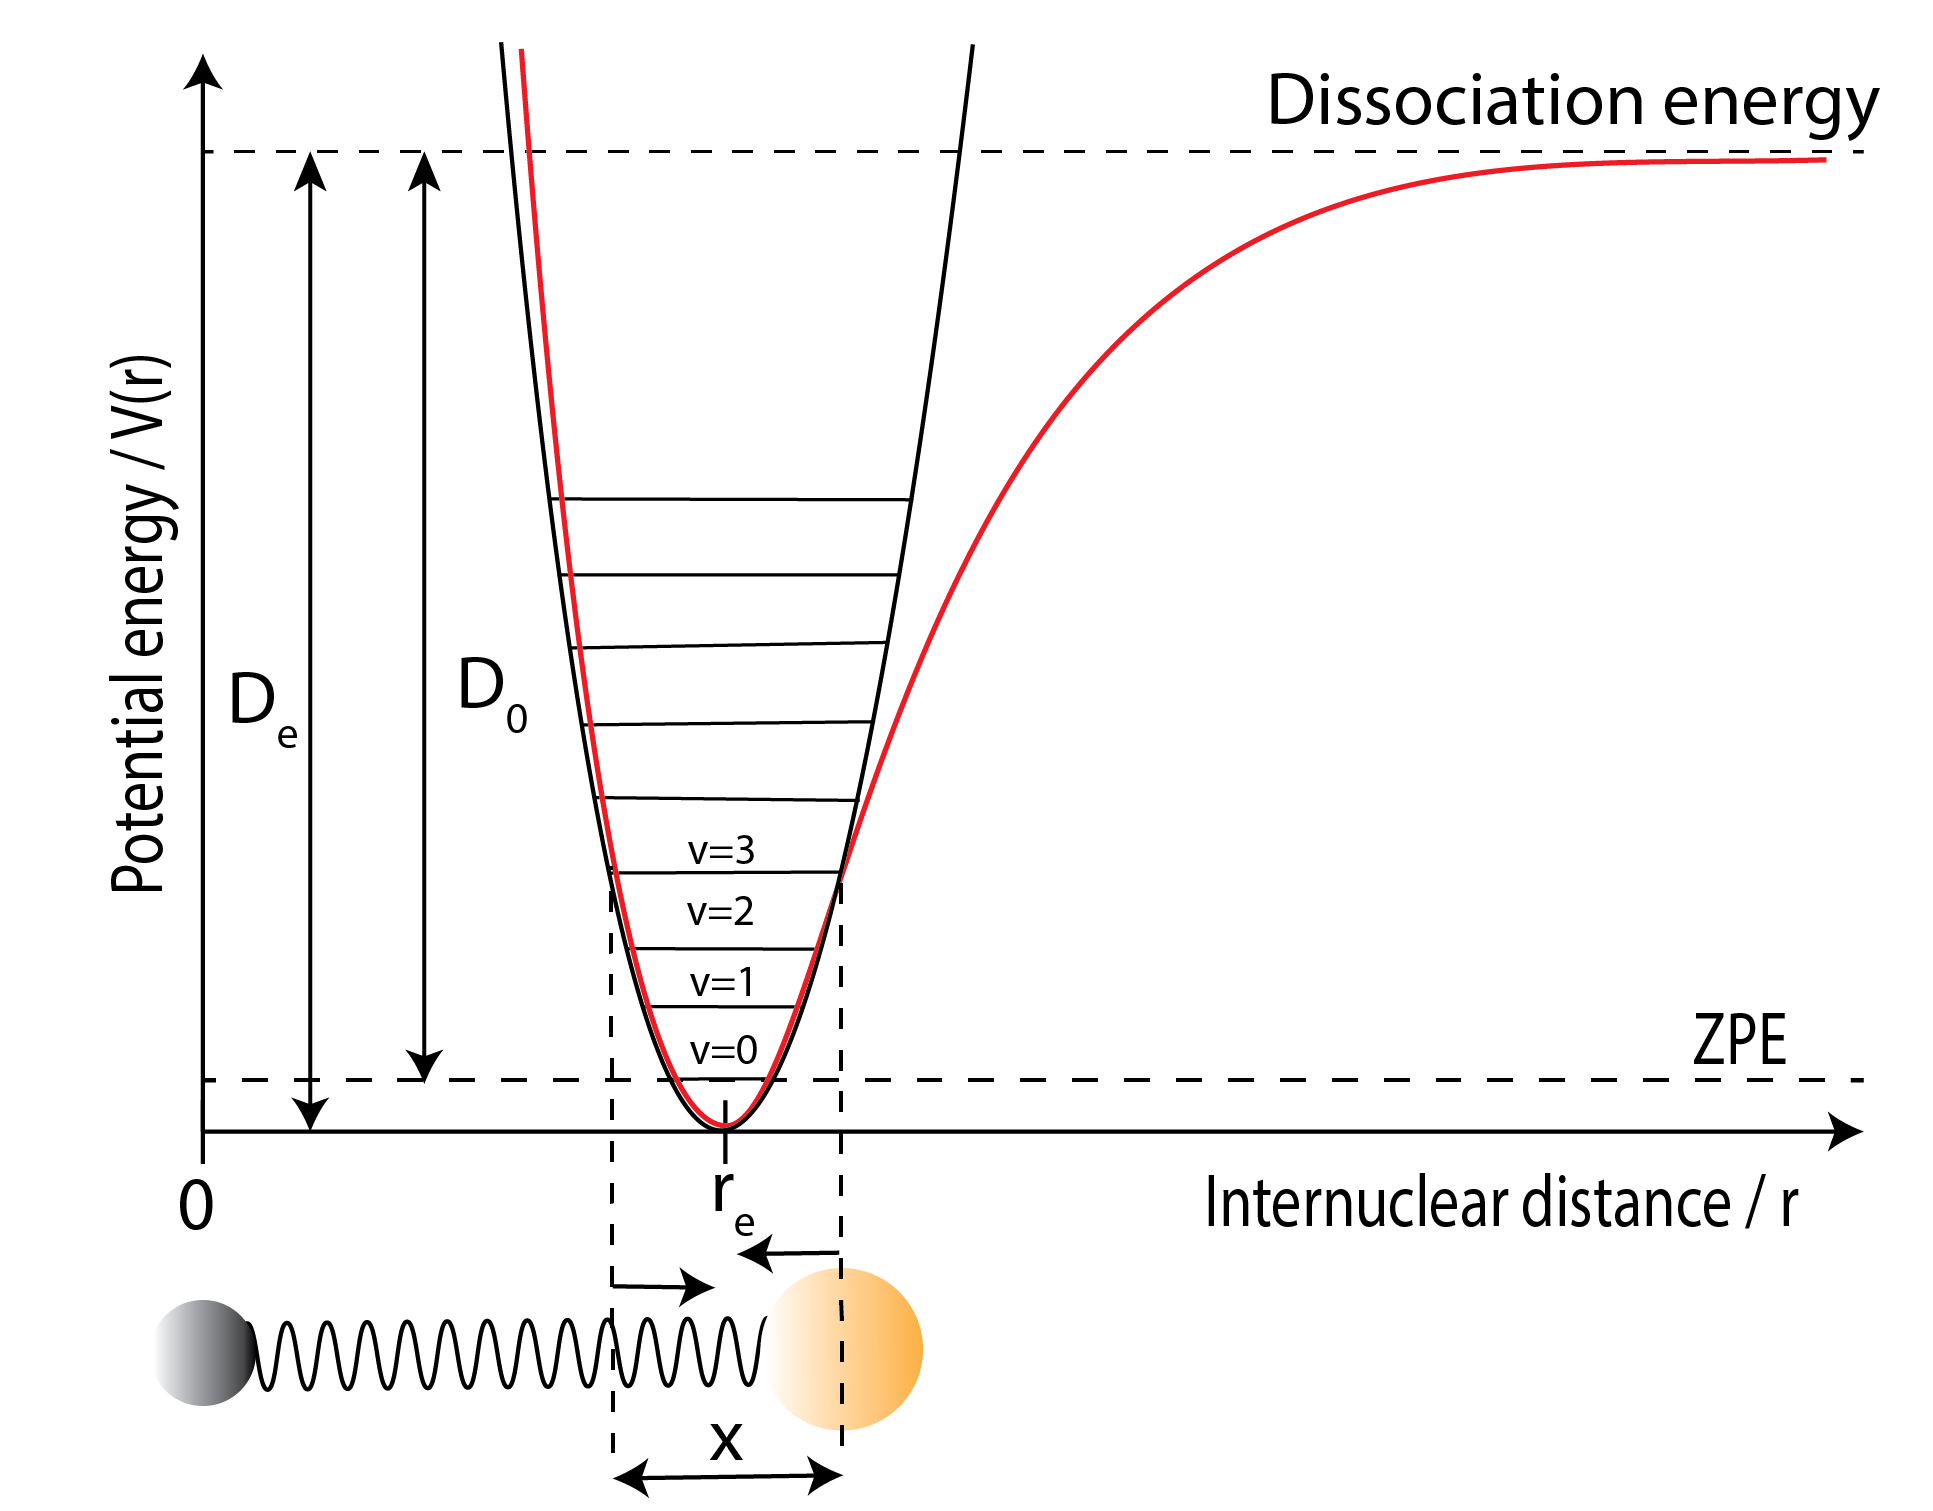
\includegraphics[scale=0.5]{figures/methods/harmonic-oscillator-01.png}
    \caption{Heteronuclear diatomic molecule (solid circles at the bottom) vibrating at energy level $v=3$. The black and red curve represent harmonic and anharmonic (Morse) potential energy curves, respectively. $r_e$ is the equilibrium bond length, $D_0$ and $D_e$ correspond to dissociation energy with and without ZPE (zero-point energy) correction, respectively. }
    \label{fig:vibration:oscillator}
\end{figure}

\subsubsection{Diatomic molecules}
\label{sec:mol-vibration:diatomic}

Assuming a simple ball and spring harmonic oscillator model as shown in Figure \ref{fig:vibration:oscillator} gives us the potential energy ($V$) from Hooke's law:
\[\text{Restoring force} = - \frac{dV(x)}{dx} = -kx\]
where $x=r-r_e$ and $k$ is force constant:

\begin{equation}
    \label{eqn:harmonic-oscillator:V(x)}
    V(x) = \frac{1}{2} k x^2
\end{equation}

Substituting, equation \ref{eqn:harmonic-oscillator:V(x)} in equations \ref{eqn:quantum:Hamiltonian} and \ref{eqn:quantum:wave-eqn}, we get the Schr\"odinger equation for 1D-oscillator:

\begin{equation}
    \label{eqn:hamiltonian-harmonic:V(x)}
    \left( -\frac{\hbar^2}{2\mu} \frac{d}{d x^2} + \frac{1}{2} k x^2 \right ) \psi_v(x) = E_v\psi_v(x)
\end{equation}
where $\mu$ is the reduced mass.

Equation \ref{eqn:hamiltonian-harmonic:V(x)} can be solved to obtain $E_v$ as given below:

\begin{equation}
    \label{eqn:vibrational-energy-Ev}
    E_v = \left( v + \frac{1}{2} \right) h \text{v} = \left( v + \frac{1}{2} \right) hc\omega
\end{equation}

where v is classical vibrational frequency, $\text{v}=\frac{1}{2\pi}\enclose{\frac{k}{\mu}}^{1/2}$, $\omega$ is vibrational wavenumber, the vibrational quantum number is $v=0, 1, 2, ...$ .


Equation \ref{eqn:vibrational-energy-Ev} shows that under the harmonic approximation, the vibrational quantum levels are equally spaced by $\hbar\omega$ and the Zero-point energy (ZPE) i.e., $E_v(v=0)=\frac{1}{2}\hbar\omega$. As shown in Figure \ref{fig:vibration:oscillator}, the ZPE is the minimum energy the molecule may have even at absolute zero temperature because of the uncertainty principle.

The energy terms are usually referred to in wavenumbers [\wn], so we can write Eq. \ref{eqn:vibrational-energy-Ev} as:

\begin{equation}
    \label{eqn:Ev-Gv}
    \frac{E_v}{hc} = \omega \enclose{v + \frac{1}{2}} = G(v)
\end{equation}

where $G(v)$ is the vibrational term value in dimensions of wavenumber, \wn.

As shown in Figure \ref{fig:vibration:oscillator}, the Morse $V(r)$ curve, the actual diatomic molecule is not accurately harmonics, especially when $r \gg r_e$. To account for anharmonicity, the harmonic oscillator term value are modified to a power series in $\enclose{v + \frac{1}{2}}$:

\[G(v) = \omega_e \enclose{v + \frac{1}{2}} - \omega_e x_e \enclose{v + \frac{1}{2}}^2 + \omega_e y_e \enclose{v + \frac{1}{2}}^3 + ...\]

where $\omega_e$ is the vibration wavenumber that a classical oscillator would have for an infinitesimal displacement from equilibrium. $\omega_e x_e$, $\omega_e y_e$, ... are the anharmonic constants.

To determine, say $\omega_e$ and $\omega_e x_e$, at least two transition wavenumbers must be obtained such as $G(1)-G(0)=\omega_0$ and $G(2)-G(1)=\omega_1$. The dissociation energy $D_e$ is given approximately (since including only $\omega_e x_e$ anharmonic term) by:
\[D_e \simeq \frac{\omega_e^2}{4\omega_e x_e}\]\\

\subsubsection{Polyatomic molecules}
\label{sec:mol-vibration:polyatomic}
The vibrational modes of an  $N$-atomic molecule are give by $3N-5$ and $3N-6$ normal vibration modes for linear and non-linear configuration, respectively.

Polyatomic vibrational modes are much more complicated to treat theoretically than diatomic. As shown in Figure \ref{fig:oscillator:water}, a simple ball-spring model with 3-atoms (H$_2$O), even if one of the nuclei is given a sudden displacement, the whole system undergoes very complicated vibrational motions (bending and stretching); this is known as Lissajous motion. For H$_2$O, we get $3(3)-6=3$ normal modes of vibrations ($v_1-v_3$). In general, a normal vibration mode is one in which all the nuclei undergo in-phase harmonic motion with the same frequency but typically with different amplitude.
\begin{figure}[!htb]
    \centering
    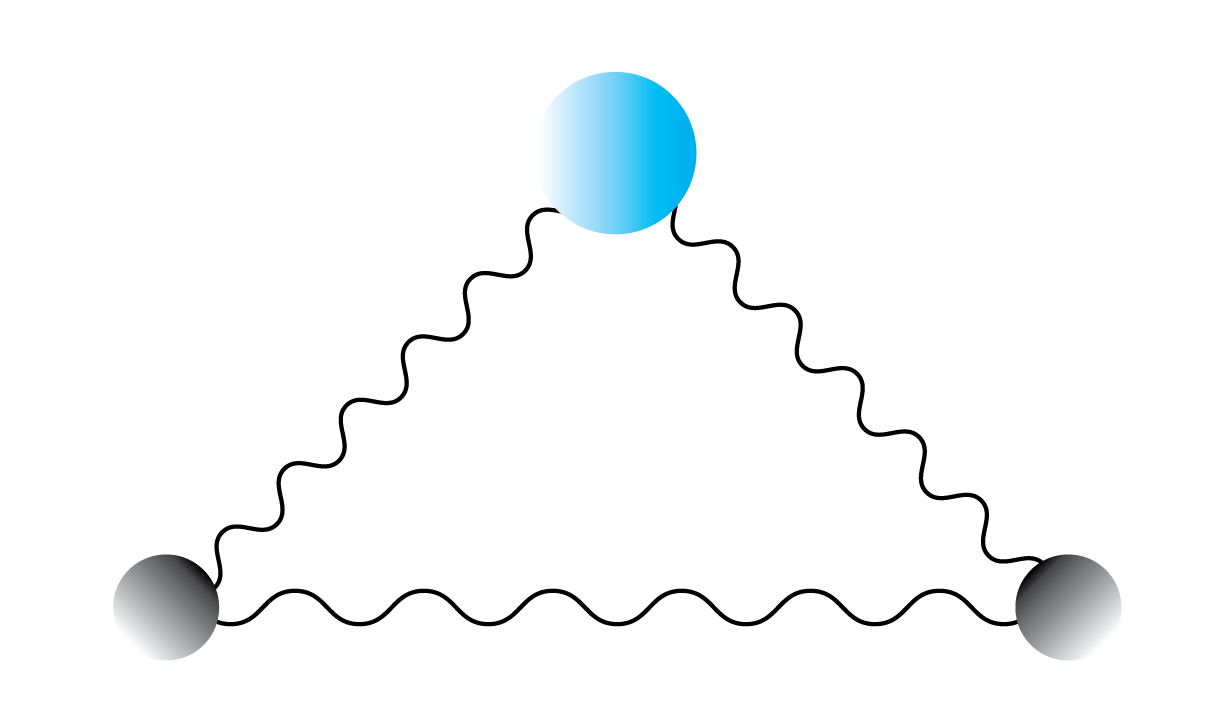
\includegraphics[scale=0.7]{figures/methods/harmonic-oscillator_polyatomic.png}
    \caption{Triatomic molecule (H$_2$O) ball-spring representation. The blue and grey circle represents oxygen and hydrogen, respectively.}
    \label{fig:oscillator:water}
\end{figure}

In polyatomic molecules, each vibrational mode can be approximated to a normal vibrational mode. With an analogous approximation from diatomic, the vibrational term value $G(v_i)$ associated with each normal vibration $i$, is given by:
\[G(v_i) = \omega_i \enclose{v_i + \frac{d_i}{2}}\]

where $d_i$ represents the degree of degeneracy.\\

\subsubsection{Selection rules}
\label{sec:mol-vibration:selection-rule}

When two vibrational states undergo absorption or emission transitions, there is usually an interaction between the molecule and the electric component of electromagnetic radiation. Therefore, the electric dipole moment ($\vec{\mu}$) determines the selection rule for vibrational transitions in the infrared spectrum.

The vibrational transition intensity is proportional to $|R_v|^2$, the square of the vibrational transition moment $R_v$, defined by:

\begin{equation}
    \label{eqn:vib:selctrion-rule}
    R_v = \int \psi^{'} \vec{\mu} \psi{''} d\tau_v
\end{equation}

where $\psi{''}$ and $\psi{'}$ are initial and final vibrational wavefunctions, respectively.\\

A transition is only allowed if the transition dipole integral is non-zero, i.e.:

\begin{align*}
    \begin{split}
        R_v &= 0 \text{ forbidden transition} \\
        R_v &\neq 0 \text{ allowed transition}
    \end{split}
\end{align*}
For diatomic molecules, within the harmonic approximation, $R_v$ is non-zero only when $\Delta v = \pm 1$. Anharmonicity can lead to $\Delta v = \pm 2, \pm 3, ...$, overtone transitions but they are generally weak.

In general, there are simple requirements for the integral of Eq. \ref{eqn:vib:selctrion-rule} to be non-zero; they are as follows.

When both $\psi{''}$ and $\psi{'}$ are non-degenerate, the symmetry species of the quantity to be integrated should be totally symmetric; that is:

\[\Gamma(\psi^{'}) \otimes \Gamma(\vec{\mu}) \otimes \Gamma(\psi^{''}) = A\]

where $A$ denotes the totally symmetric species of any non-degenerate point group, and $\Gamma$ stands for symmetry representation.

For degenerate states:
\[\Gamma(\psi^{'}) \otimes \Gamma(\vec{\mu}) \otimes \Gamma(\psi^{''}) \supset A\]

A brief overview of molecular vibration for diatomic and polyatomic molecules has been discussed, along with the selection rule for observing IR active vibrational transition modes using quantum mechanics. The following section deals with the quantum mechanical theory of molecular rotation.

\subsection{Molecular rotation}
\label{sec:mol-rotation}

Molecules have electronic and vibrational energy due to the motion of electrons and nuclei, respectively. Furthermore, they have rotational energy due to the overall rotation of the molecule. Like electronic and vibrational, rotational energy is quantized and generally has very small energies compared to the former.

\begin{figure}[!htb]
    \centering
    
    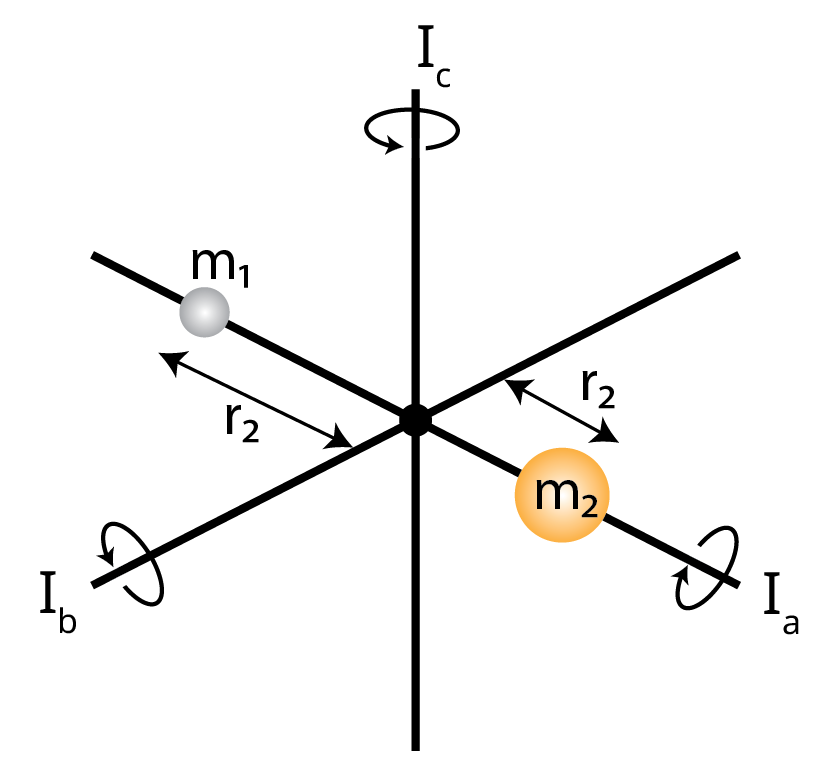
\includegraphics[scale=0.7]{figures/methods/rotation-rotor_linear.png}
    \caption{Rotation of linear molecule (heteronuclear diatomic) w.r.t principal rotational axis $a, b$ and $c$, with corresponding moment of inertia $I_a, I_b$ and $I_c$, respectively ($I_a$=0, $I_b$=$I_c$ for linear and diatomic molecules). $m$ and $r$ represent the mass of the atom and the distance to the rotating axis, respectively. The centre of mass lies at the origin.}
    \label{fig:rotor:diatomic}
\end{figure}

The molecules are classified according to their principal moments of inertia, $I_a, I_b$ and $I_c$, i.e., the moment of inertia along the principal rotational axis $a, b$ and $c$, respectively. The corresponding rotational constants are denoted as $A, B$ and $C$, respectively. The principal axes are perpendicular to each other and pass through the molecule's centre of mass (as shown in Figure \ref{fig:rotor:diatomic}). In general, the axes are conventionally defined such that: 

\begin{equation}
    \label{eqn:Iabc-reltion}
    I_a \leq I_b \leq I_c
\end{equation}

The moment of inertia, $I$, is defined as 

\begin{equation}
    \label{eqn:moment-of-inertia}
    I = \sum_i m_i r_i^2
\end{equation}

where $m_i$ and $r_i$ correspond to mass and distance to the rotating principal axis of atom $i$, respectively.

The main classifications are linear and non-linear molecules, while the latter is further divided, as will be briefly discussed in the following sections.

\subsubsection{Linear molecules}
\label{sec:mol-rotation:linear}

With a rigid rotor approximation, i.e., the bonds are rigid rods and molecule as a rigid rotor, the angular momentum is given by:

\[P_J = [J(J+1)]^{\frac{1}{2}} \hbar\]
where the rotational number $J=0, 1, 2, 3, ...$ .\\

In the presence of an electric or magnetic field,

\begin{equation}
    \label{eqn:rotation:MJ}
    (P_J)_z = M_J \hbar
\end{equation}

where, subscript $z$ represent z-axis component and $M_J = J, J-1, ..., -J$. This indicates that in the absence of an electric or magnetic field, each rotational level has $2J+1$ degenerate states.\\

The rotational energy ($E_r$) for a diatomic or linear polyatomic molecule can be solved using Eq. \ref{eqn:quantum:wave-eqn} and is given by:

\begin{equation}
    \label{eqn:rotational-energy-Er}
    E_r = \frac{h^2}{8\pi^2 I_b} J (J+1)
\end{equation}

The rotational energy in frequencies [Hz] can be defined using Eq. \ref{eqn:rotational-energy-Er}:

\begin{equation}
    \label{eqn:rotational-energy-FJ}
    F(J) = \frac{E_r}{h} = \frac{h}{8\pi^2 I_b} J(J+1) = BJ(J+1)
\end{equation}

where $F(J)$ is the rotational term values and $B$ is the rotational constant.\\
Only $B$ rotational constants are involved for linear molecules since as shown in Figure \ref{fig:rotor:diatomic}, $I_a=0$ and $I_b=I_c$.\\

The rigid rotor approximation does not hold true, especially in higher $J$ energy levels, because the chemical bonds expand due to centrifugal forces from molecular rotation. The expansion due to centrifugal force is included in equation \ref{eqn:rotational-energy-FJ} such that

\begin{equation}
    \label{eqn:rotational-energy-FJ-DJ}
    F(J) = BJ(J+1) -DJ^2(J+1)^2 + ...
\end{equation}

where $D$ is the centrifugal distortion constant. Eq. \ref{eqn:rotational-energy-FJ-DJ} also indicates that further higher-order terms may be included.

\subsubsection{Non-linear molecules}
\label{sec:mol-rotation:non-linear}
The non-linear molecules are further classified based on the principal moment of inertia. Analogous to $B$ rotational constant for linear molecule (Eq. \ref{eqn:rotational-energy-FJ}), the rotational constants $A, B$ and $C$ are given by:

\begin{equation}
    \label{eqn:rotational-constants}
    A=\frac{h}{8\pi^2 I_a};\ B=\frac{h}{8\pi^2 I_b};\ C=\frac{h}{8\pi^2 I_c}
\end{equation}

with units of frequency [Hz].\\

\textbf{Symmetric top: } It has two equal principal moments of inertia which corresponds to two possibilities: (a) $I_a < I_b = I_c$ and (b) $I_a = I_b < I_c$, these are called prolate and oblate, respectively. In symmetric tops, a second rotational quantum number $K=0, 1, 2, ..., J.$ is introduced in addition to $J$; therefore, Eq. \ref{eqn:rotational-energy-FJ} becomes

\begin{align}
    F(J, K) &= BJ(J+1) + (A-B)K^2\ \text{(prolate)} \label{eqn:rotational-energy-FJ-AKJ}\\
    F(J, K) &= BJ(J+1) + (C-B)K^2\ \text{(oblate)} \label{eqn:rotational-energy-FJ-CKJ}
\end{align}

The equations \ref{eqn:rotational-energy-FJ-AKJ} and \ref{eqn:rotational-energy-FJ-CKJ} indicate that for a particular value of $J$, the energy levels diverge and converge for a prolate and oblate symmetric tops, respectively. Since from Eq. \ref{eqn:Iabc-reltion} and \ref{eqn:rotational-constants}, we have $A \geq B \geq C$.\\

When the effect of centrifugal distortion is included, Eq. \ref{eqn:rotational-energy-FJ-AKJ} becomes (for prolate),
\begin{equation}
    \label{eqn:rotational-energy-FJ-KJ}
    F(J, K) = BJ(J+1) + (A-B)K^2 - D_J J^2(J+1)^2 - D_{JK} J(J+1)K^2 - D_K K^4
\end{equation}

where there are now three centrifugal constants $D_J, D_{JK}$ and $D_K$.\\

\textbf{Spherical top: }It has all three principal moments of inertia equal, i.e., $I_a = I_b = I_c$. Therefore, the rotational term value follows the same as the equation for diatomic or linear polyatomic \ref{eqn:rotational-energy-FJ} and \ref{eqn:rotational-energy-FJ-DJ} (Section \ref{sec:mol-rotation:linear}).\\

\textbf{Asymmetric top: } It has all three principal moments of inertia unequal, i.e., $I_a \neq I_b \neq I_c $. Generally, the vast majority of molecules are asymmetric tops. But unfortunately, there are no analytical formulae for rotational term values for asymmetric tops molecules. $J$ is still a good quantum number, but $K$ is not, i.e., it does not take integral values. Therefore, only approximate expressions are derived, i.e., to approximate the molecule to either prolate or oblate near-symmetry top, such as:

\begin{align*}
    \begin{split}
        F(J, K) &\simeq B^* J(J+1) - (A-B^*)K^2\ \text{(near-prolate)} \\
        F(J, K) &\simeq B^* J(J+1) - (C-B^*)K^2\ \text{(near-oblate)}
    \end{split}
\end{align*}

where $B^*$ is equal to $\frac{1}{2} (B+C)$ for prolate and $\frac{1}{2} (A+C)$ for oblate rotor.

Since $K$ is not strictly a good quantum number and the $F(J, K)$ is only approximated.

\subsubsection{Selection rules}
\label{sec:mol-rotation:selection-rule}

Similar to the vibrational selection rule as discussed in Section \ref{sec:mol-vibration:selection-rule}, the rotational selection rule is determined from the rotational transition moment, $R_r$, defined as:

\[R_r = \int \psi_r^{'} \Vec{\mu} \psi^{''}\]

The rotational selection rule constitutes the condition for which $R_r$ is non-zero.\\

The selection rule:\\

for linear molecules and spherical top

\begin{enumerate}
\item $\Delta J = \pm 1$
\end{enumerate}

for symmetric top

\begin{enumerate}
\item $\Delta J = \pm 1$
\item $\Delta K = 0$
\end{enumerate}

for the asymmetric top

\begin{enumerate}
\item $\Delta J = 0, \pm 1$
\end{enumerate}

In addition to the above rules, all molecules must have a permanent electric dipole moment ($\Vec{\mu} \neq 0$) to observe rotational transition, and in the presence of the electric or magnetic field $\Delta M = 0, \pm 1$ (see Eq. \ref{eqn:rotation:MJ}).\\

The next section discusses relevant technical details for quantum chemical calculation employed in this thesis work.

\subsection{Quantum chemical calculations}
\label{sec:QC-calculations}
The molecular vibration and rotation laboratory spectroscopic studies reported in this work are supported by quantum chemical calculations as described in Section \ref{sec:mol-vibration} and \ref{sec:mol-rotation}. This section briefly discusses the methods and programs used to employ quantum chemical calculations.

Initially, a potential energy surface is computed to characterize the molecular ion of interest, and energetically stable structures are derived and structurally optimised. These investigations are performed at the coupled-cluster singles and doubles (CCSD) level augmented by a perturbative treatment of triple excitations, CCSD(T) \cite{raghavachari_fifth-order_1989}, in combination with atomic natural orbital (ANO0, ANO1, and ANO2) basis sets from Alml\"of and Taylor \cite{almlof_general_1987, almlof_atomic_1991} as well as the correlation-consistent valence basis set cc-pVDZ \cite{dunning_gaussian_1989} in the frozen core (fc) approximation. The equilibrium geometries have been calculated using analytic gradient techniques  \cite{watts_open-shell_1992}.

Vibrational modes of molecular ions of interest are further investigated by computing harmonic frequencies using numerical differentiation of gradients \cite{lee_analytic_1991, watts_coupledcluster_1993}. Second-order vibrational perturbation theory (VPT2) \cite{mills_32_1972} has been employed for anharmonic calculations. All CCSD(T) calculations have been carried out using the CFOUR program package  \cite{matthews_coupled-cluster_2020,harding_parallel_2008}.

The influence of the rare gas tag on the IRPD spectrum is further investigated by computing interaction energies (using either CFOUR \cite{matthews_coupled-cluster_2020} or PSI4 \cite{smith_psi4_2020} program) as well as harmonic frequencies of the ionic complexes. For the complexes, the Basis Set Superposition Errors (BSSE) \cite{liu_accurate_1973} are addressed using i) the counter-poise (CP) method introduced by Boys and Bernardi \cite{boys_calculation_1970}, i.e. by calculating CP-corrected CCSD(T) interaction energies at each geometry, and ii) higher-order symmetry-adapted perturbation theory, SAPT2+3 \cite{jeziorski_perturbation_1994, hohenstein_density_2010}. 

Measured pure rotational and vibrational transitions (see Chapter \ref{chapter:CO+}) are fitted with an effective Hamiltonian approach using the Pgopher program \cite{western_pgopher_2017} to derive molecular spectroscopic constants. Further computational details specific to certain ionic species are reported in their respective chapters in detail. The next section focuses on experimental technical details such as determining number density.
